% celo-feedback-template.tex  -- Deploying a contract on the Celo blockchain
% 2021-01-14
\documentclass[a4paper,11pt]{article}
\usepackage{geometry}
\usepackage{xurl}
\usepackage{graphicx}
\title{Celo/BAF Celo for Eth Devs Feedback}
\author{Charlie Timmins\\
  \url{https://github.com/catimmins/celo-feedback}}
\date{\begin{flushright}Jan. 2020\end{flushright}}

\begin{document}
\maketitle

\section*{Introduction}
I'm a software, and more recently Ethereum, developer working in a
blockchain-based startup and am personally interested in how blockchain
technologies can be used to preserve and transmit information. My previous
experience is in writing smart contracts written in Solidity and I'm excited to
explore how this translates to the Celo protocol.

\section*{Process}
\emph{List the actions that you took during the exercise and include screenshots
  of problems your encountered}
\\\\
I began by become familiar with Celo through the documentation at
\url{https://docs.celo.org/}.  The layout of these pages was clear and I
appreciated that the links to start using the testnet immediately followed the
highlighted features as I was keen to get started after reading these.  The
documentation strongly encouraged me to use the Android client, however I chose
to generate an account on the command line using the Docker container.  I was
able to do this, add funds to the account, and verify the balance using the
Blockscout without any difficulty.\\


% Sending Celo
It's essential in development that basic operations on the blockchain can be
performed programatically so I next opened the developer docs to explore how
accounts can be created in this way.  The helloCelo tutorial at
\url{https://docs.celo.org/developer-guide/start/hellocelo} provided a simple,
but effective introduction to how the Celo blockchain might be used in practice
and was clear for anyone familiar with JavaScript.  Using it I was able to
create another account send a minute amount of CELO to the testnet account I had
created earlier [Fig. \ref{fig:sending}].  I did note that there didn't appear
to be any way to request funds from the faucet using the JS SDK.  I assume this
is to prevent it being flooded by a deluge of automated requests, however I
couldn't see any alternatives for automated testing.\\
% interesting that the faucet can't be used programatically -- or at least I couldn't find out how

\begin{figure}[hbt!]
  \centering
  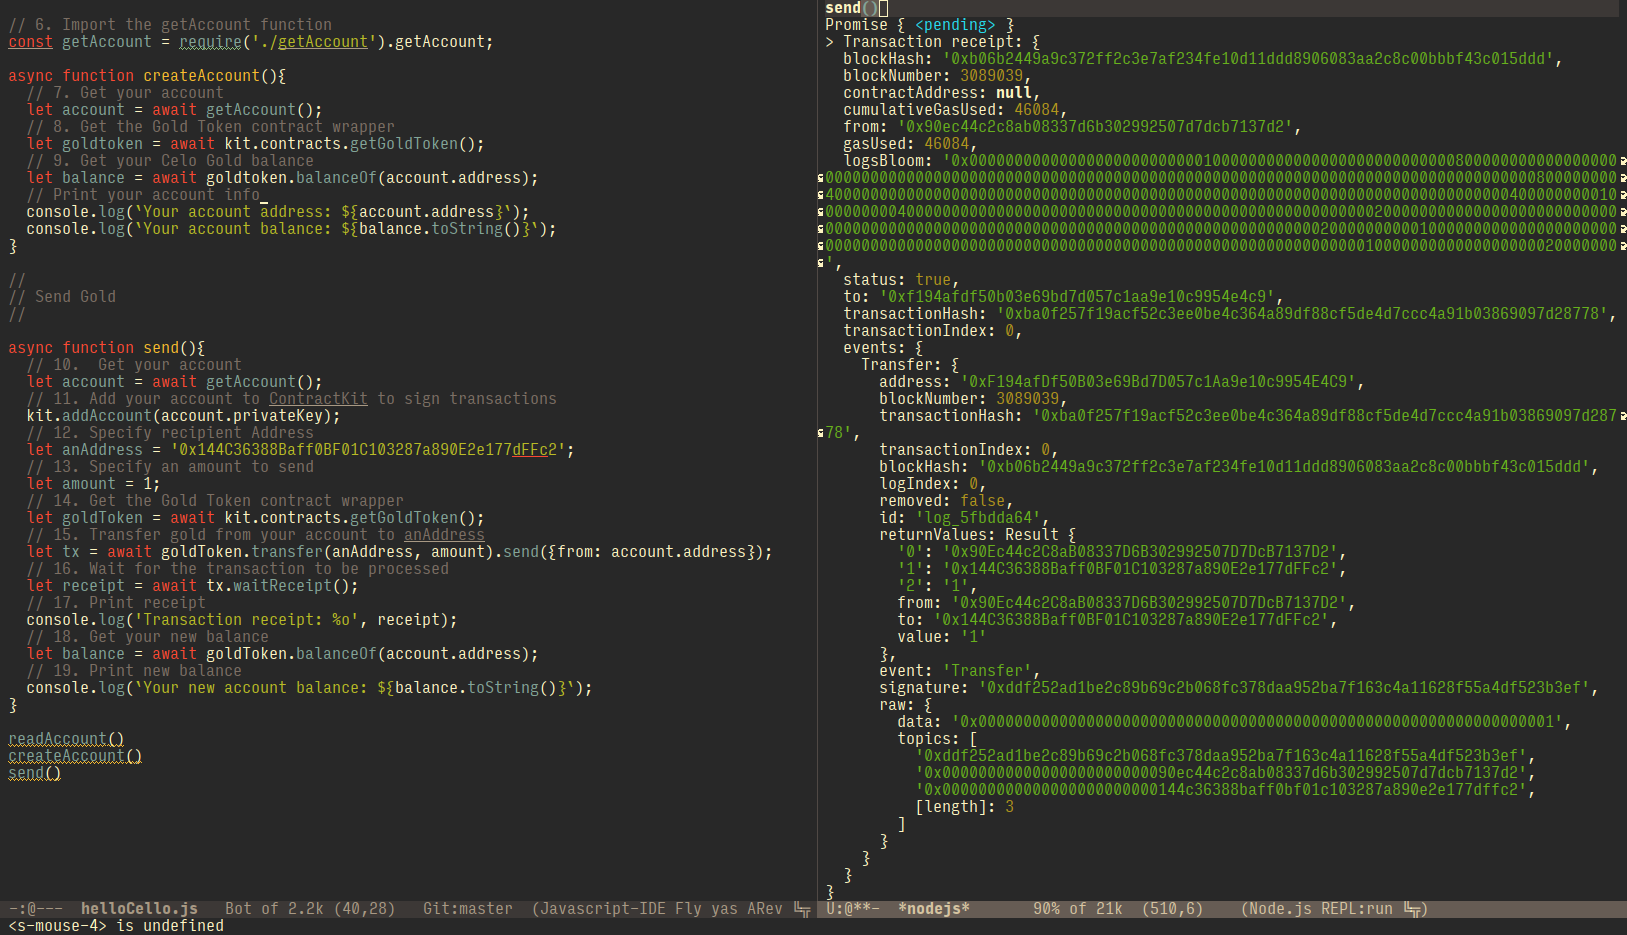
\includegraphics[width=\textwidth]{sending}
  \caption{Sending CELO}
  \label{fig:sending}
\end{figure}

% Deploy a contract (forno)
At this point I was onboard the Celo network with a funded testnet account and
sought to start deploying contracts.  I chose to follow the tutorial on
deploying a contract using a remote node via Forno as I have experience
working this way on Ethereum and wished to compare the workflow on Celo.  I was
pleased to discover that there's very little difference in the process and many
Ethereum tools can be used unmodified.  In addition to the example contract
provided I was able to deploy a simple contract I had written some time ago for
Ethereum without any changes and using only the short deployment scripts
provided [Fig. \ref{fig:messageboard}].\\

\newpage

\begin{figure}[hbt!]
  \centering
  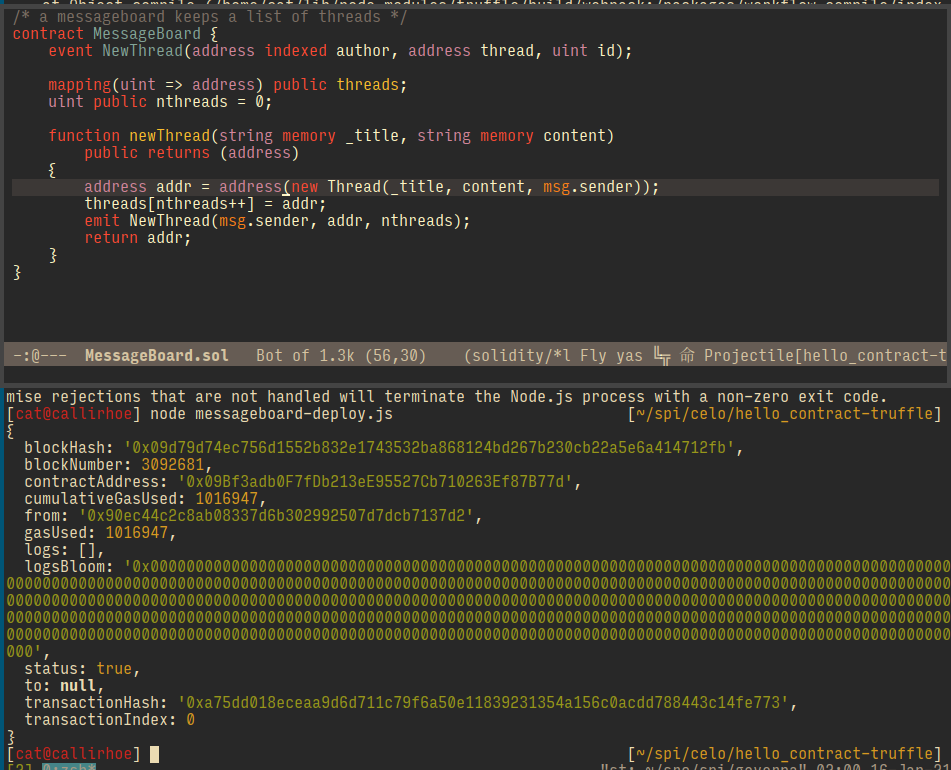
\includegraphics[width=0.6\textwidth]{deploy-messageboard}
  \caption{Deploying a minimal blockchain messageboard}
  \label{fig:messageboard}
\end{figure}


\subsection*{Deploying Complex Contracts}
I followed this up by deploying a more complicated set of contracts to assess
what adaptions, if any, would be required to move to Celo.  I chose the
Chainlink ERC20 token and oracle as
% add github link
as it's a very mature project tightly integrated with the Ethereum platform.  I
expected that this would expose deficiencies in Celo, however I was very
pleasantly surprised that it was only a matter of configuring truffle.  Far more
time was spent tracking down dependencies and figuring out the structure of
Chainlink than working with Celo.  Deployment seceded without any problems as
seen in [Fig. \ref{fig:chainlink}]
The Oracale can be found at \verb|0x8c9373c7ad3E1b3078EEde0344216328E48cD0bA|
and associated LINK token contract at
\verb|0x4577A1D712330f92E7D7105F947696bf2eeE51c0|, both on Alfajores.

\begin{figure}[hbt!]
  \centering
  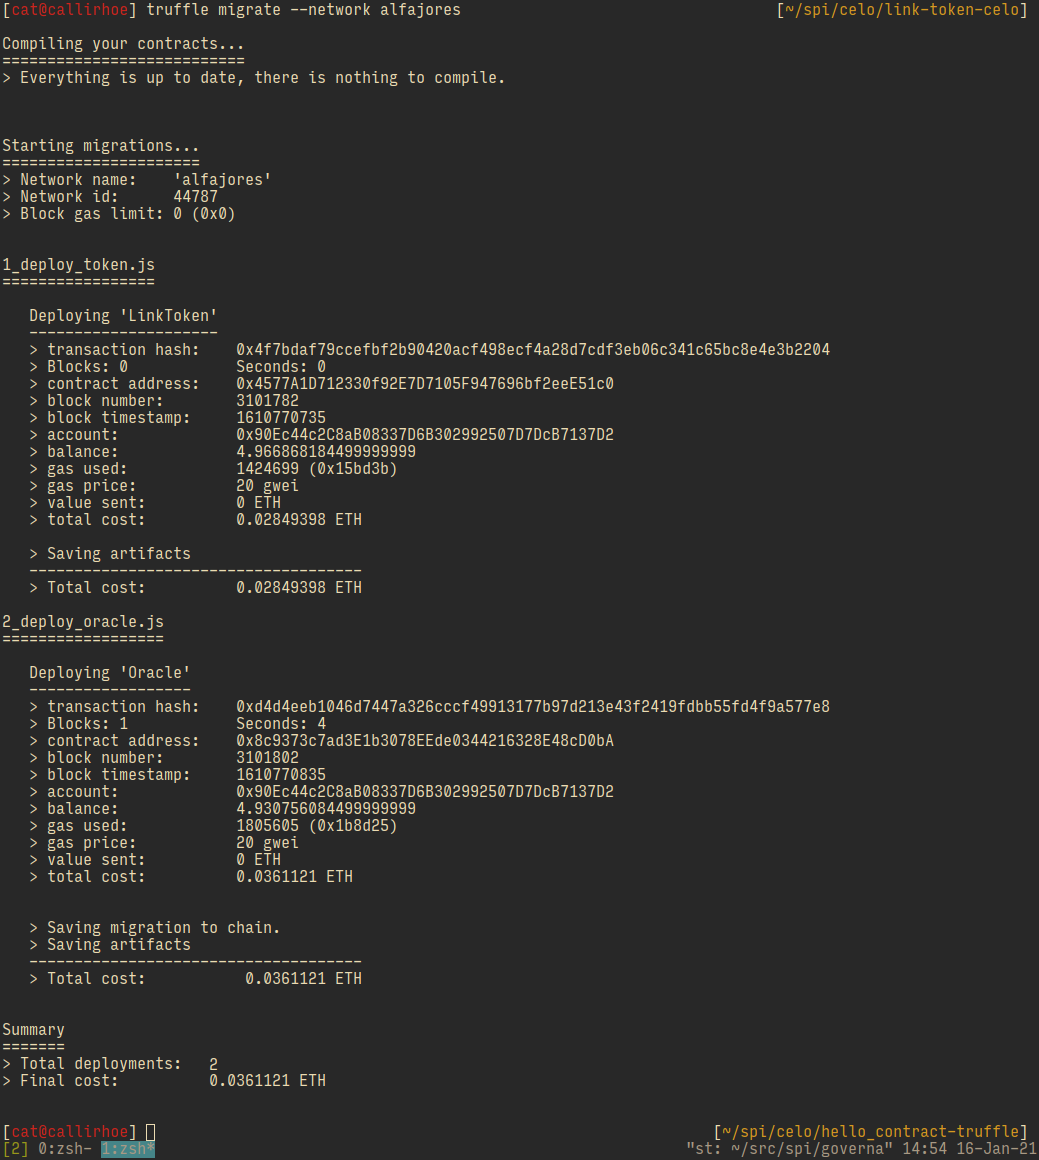
\includegraphics{deploy-chainlink}
  \caption{Deploying LINK and Oracle}
  \label{fig:chainlink}
\end{figure}

\subsection*{I really liked:}
\begin{itemize}
\item Compatibility with Ethereum
\item Documentation encourages users to start exploring the network straight
  away.
\item The Javascript SDK appears to be robust and provides a large amount of
  common functionality.
\end{itemize}
\subsection*{I had a hard time with:}
\begin{itemize}
\item The documentation often reminds the reader that Celo is not 100\%
  compatible with Ethereum without elaborating on what the differences are or
  where they lie.  This led to some apprehension in using Ethereum tools and
  handling potential errors.
\item Being able to use Ethereum tooling is a definite advantage, however it can
  lead to a confusing mismatch of information, Truffle still reports value and
  gas prices in ETH and gwei, respectively.  I was unsure what these meant in
  terms of CELO.
\end{itemize}
\subsection*{I encountered these errors along the way:}
\begin{itemize}
\item There was some inconsistency in the examples that initially disoriented
  me.  The helloCelo tutorial is very hands on, encouraging the user to fill in
  each line according to the given instructions, while the remote deployment
  tutorial is really just a matter of pulling a repository and running the code.
  They explain creating an address on Alfajores in very different terms to the
  point where I initially didn't realise I already had the required account.
\item The Celo for Ethereum developers document provides a good high-level
  overview of the differences in the protocol, however it doesn't provide any
  examples or links on how the unique features can be used in contracts.
\end{itemize}
\section*{General Impression}
\subsection*{How long did this take you?}
I spent roughly 5-7 hours reading through the Celo documentation, testing code,
and deploying contracts.  This is about right for getting acquainted with a new
technology in my experience.
\subsection*{How could this exercise be improved?}
There are huge amount of features and tools listed in the Celo documentation,
some of which I didn't get the opportunity to go through.  A broader range
of tasks could have better demonstrated what Celo has to offer.  In particular I
was very impressed with the quality of the SDK and would have liked to explore
how it can be used to build blockchain-based applications.
\end{document}
